\documentclass{article}

\usepackage[T1]{fontenc}
\usepackage[utf8]{inputenc}
\usepackage{lmodern}
\usepackage{amsmath}
\usepackage{graphicx}


\author{Sigrid Videm}
\title{Project 1}

\begin{document}
\maketitle
\tableofcontents % for a table of contents

\section{Abstract} 
The aim of this project was to explore different methods for solving the second order differential equation $-u''(x)=f(x)$, and to investigate the loss of numerical precision assosiated with these methods. To solve the equation, I have have used the three point formula for the second derivative, and rewritten the equation as an equation of the type Av=q. The matrix A is a tridiagonal matrix, and I developed a general  algorithm for doing row reduction on tridiagonal matrices. Later, I used the fact that the elements of A are either -1 or 2, and found an analytic expression for for the row reduction of such a matrix. At last, I used the built-in LU decomposition of Python. For these three methods I compared the computing time, and number of FLOPs. 

To look at the loss of numerical precision, I used the most effective algorithm, and made a function calculating the relative error for different step lengths. Using double precision, I found no considerable loss of numerical precision, but I had some suprising results regarding the slope of the error as a function of step length. The error was of order $h^{-1}$. These reults are probably linked, but I have not found an explanation. 
\section{Introduction}
In the methods section, I will show how the three point formula for the second derivative can be used to discretize the equation $u''(x)=-f(x)$, and how to rewrite this set of equations as a matrix equation. I will use Gaussian elimination to make an algorithm for solving this equation. The Gaussian elimination gives analytical result for the diagonal elements and for the vector v. This gives rise to an algorithm that does not include matrix operations. 
The results and Discussion section includes plots of the solution found by the general algoritm, plots of the relative error of the second algorithm, and a discussion on loss numerical precision. There is also a table comparing the CPU time of the different methods, and a discussion of how this relates to the number of FLOPs. 
\section{Method}
\subsection{Discretizing the second order differentail equation}

The three point formula:
$$
f_i''=\frac{f_{i+1}+f_{i-1}-2f_i}{h^2}+O(h^2)
$$
Let $i \in [1,2,3,4]$, and $x_0=x_5=0$
$$
f_1''=\frac{f_{2}+f_{0}-2f_1}{h^2}
$$
$$
f_2''=\frac{f_{3}+f_{1}-2f_2}{h^2}
$$
$$
f_3''=\frac{f_{4}+f_{2}-2f_3}{h^2}
$$
$$
f_4''=\frac{f_{5}+f_{3}-2f_4}{h^2}
$$

can be rewritten as
$$
\begin{bmatrix}
2 & -1 & 0 & 0 \\
-1 & 2 & -1 & 0 \\
0 & -1 & 2  & -1 \\
0 & 0 & -1 & 2 \\
\end{bmatrix}
\begin{bmatrix}
f_1\\
f_2\\
f_3\\
f_4\\
\end{bmatrix}
=h^2
\begin{bmatrix}
f_1''\\
f_2''\\
f_3''\\
f_4''\\
\end{bmatrix}
$$


The equation I want to solve is $u''(x)=-100e^{-10x}$. The elements of the solution vector are $f_i''=-h^2 100e^{-10i}$

One exact solution of this equation is $u(x)=1-(1-e^{-10})x-10e^{-10x} $. I will use this solution for comparing the exact solution and the numerical , and to calculate the relative error. 

\subsection{Gaussian elimination on a tridiagonal matrix}
Gaussian elimination on a tridiagonal matrix, exemplified by a 4x4 matrix: 

$$
\begin{bmatrix}
a_{11} & a_{12} & 0 & 0 \\
a_{21} & a_{22} & a_{23} & 0 \\
0 & a_{32} & a_{33} & 0 \\
0 & 0 & a_{43} & a_{44} \\
\end{bmatrix}
v=
\begin{bmatrix}
f_1\\
f_2\\
f_3\\
f_4\\
\end{bmatrix}
$$
Gaussian elimination on the second row:
$$
\begin{bmatrix}
a_{11} & a_{12} & 0 & 0 \\
a_{21}-a_{11}\frac{a_{21}}{a_{11}} & a_{22} -a_{12}\frac{a_{21}}{a_{11}} & a_{23}-0 & 0 \\
0 & a_{32} & a_{33} & 0 \\
0 & 0 & a_{43} & a_{44} \\
\end{bmatrix}
v=
\begin{bmatrix}
f_1\\
f_2-f_1\frac{a_{21}}{a_{11}}\\
f_3\\
f_4\\
\end{bmatrix}
$$
repeat this for all rows, and you get an upper triangular matrix:
$$
\begin{bmatrix}
a_{11} & a_{12} & 0 & 0 \\
0 & b_{22} & a_{23} & 0 \\
0 & 0 & b_{33} & a_{43} \\
0 & 0 & 0 & b_{44} \\
\end{bmatrix}
v=
\begin{bmatrix}
f_1\\
\tilde{f_2}\\
\tilde{f_3}\\
\tilde{f_4}\\
\end{bmatrix}
$$

Gaussian elimination on the elements above the diagonal:
$$
\begin{bmatrix}
a_{11} & a_{12} & 0 & 0 \\
0 & b_{22} & a_{23} & 0 \\
0 & 0 & b_{33} & a_{43}-b_{44}\frac{a_{43}}{b{44}} \\
0 & 0 & 0 & b_{44} \\
\end{bmatrix}
v=
\begin{bmatrix}
f_1\\
\tilde{f_2}\\
\tilde{f_3}-\tilde{f_4}\frac{a_{43}}{b_{44}}\\
\tilde{f_4}\\
\end{bmatrix}
$$

Gaussian elimination on the elements above the diagonal:
$$
\begin{bmatrix}
a_{11} & 0 & 0 & 0 \\
0 & b_{22} & 0 & 0 \\
0 & 0 & b_{33} & 0 \\
0 & 0 & 0 & b_{44} \\
\end{bmatrix}
v=
\begin{bmatrix}
q_1\\
q_2\\
q_3\\
\tilde{f_4}\\
\end{bmatrix}
$$
The solution:
$$
v=
\begin{bmatrix}
\frac{a_{11}}{q_1}\\
\frac{b_{22}}{q_2}\\
\frac{b_{33}}{q_3}\\
\frac{b_{44}}{\tilde{f_4}}\\
\end{bmatrix}
$$
I used this algoritm on the matrix A and vector f, where $f_i =h^{2}(100\exp{-10i})$
$$
A=
\begin{bmatrix}
2 & -1 & 0 & 0 \\
-1 & 2 & -1 & 0 \\
0 & -1 & 2  & -1 \\
0 & 0 & -1 & 2 \\
\end{bmatrix}
$$
The results are given as plots in the next section, for $A \in R^{10x10}$,$A \in R^{100x100}$, $A \in R^{1000x1000}$
\subsection{Specialized algorithm}
For developing the specialized algorithm, I used the fact that all the diagonal elements have value 2, and the elments immediately above and belove the diagonal have elements -1. In this case, the forward substitution gives analytical expressions for the elements along the diagonal, $b_{ii}$, and  for the elements $v_i$: 
$$ b_{ii} = \frac{i+2}{i+1}$$
$$v_i = f_i+\frac{v_{i-1}}{b_{ii}}$$
I found the solution of the equation by backward substitution:
$$
x_i= \frac{v_i+x_{i+1}}{b_{ii}}
$$
To check the efficiency of this new algorithm, compared the CPU time for this algoritm and the previous one. I used 10 000 grid points, because this was the largest dimension possible the N times N matrix in Python. The results are presented in a table in the next section, along with the CPU time of the built in solve function from Python. The CPU-time in the table is the mean of 5 runs.

\subsection{Relative error}
To calculate the relative error, I used the specialized algorithm to calculate a solution $v$, and the exact solution $u$. I calculated the relative error $\epsilon_i = \frac{v_i-u_i}{u_i}$ for all N elements, except for the end elements, because $x_N=u_N$, and found the maximum value for the relative error. I did this for $ N=10, 100, .., 10^{7}$  grid points. The maximum error as a function of step length $h=1/N$ is shown as a plot in the next section. This plot shows no loss of numerical precision, and the slope is approximately 1. I investigated this further, by setting the precision to 32, rather that 64, whitch is the default precision i Python. Then, I made the same plot. 


\section{Results and Discussion}
\subsection{The numerical solution}
The figures 1-3 show the exact solution $u(x)=1-(1-e^{-10})x-10e^{-10x} $ (red line) of the differential equation $-u''(x)=f(x)$, along with the numerical solution found by the method described in section 3.1 (blue line). The end points $x=0$ and $x=0$ are not included, because the matrix representation of the set of equations does not include this point. However, when N is increased, the function values gets closer to zero at both ends, and ths is consistent with the boundary conditions $u(0)=u(1)=0$. By comparing the curves, it is clare that with 1000 grid points, the exact solution looks very similar to the exact one, and this indicates that the algorithm used here for solving the second order differential equation is quite good. How good it is, is the subject of the next paragraph. 
\begin{figure}
  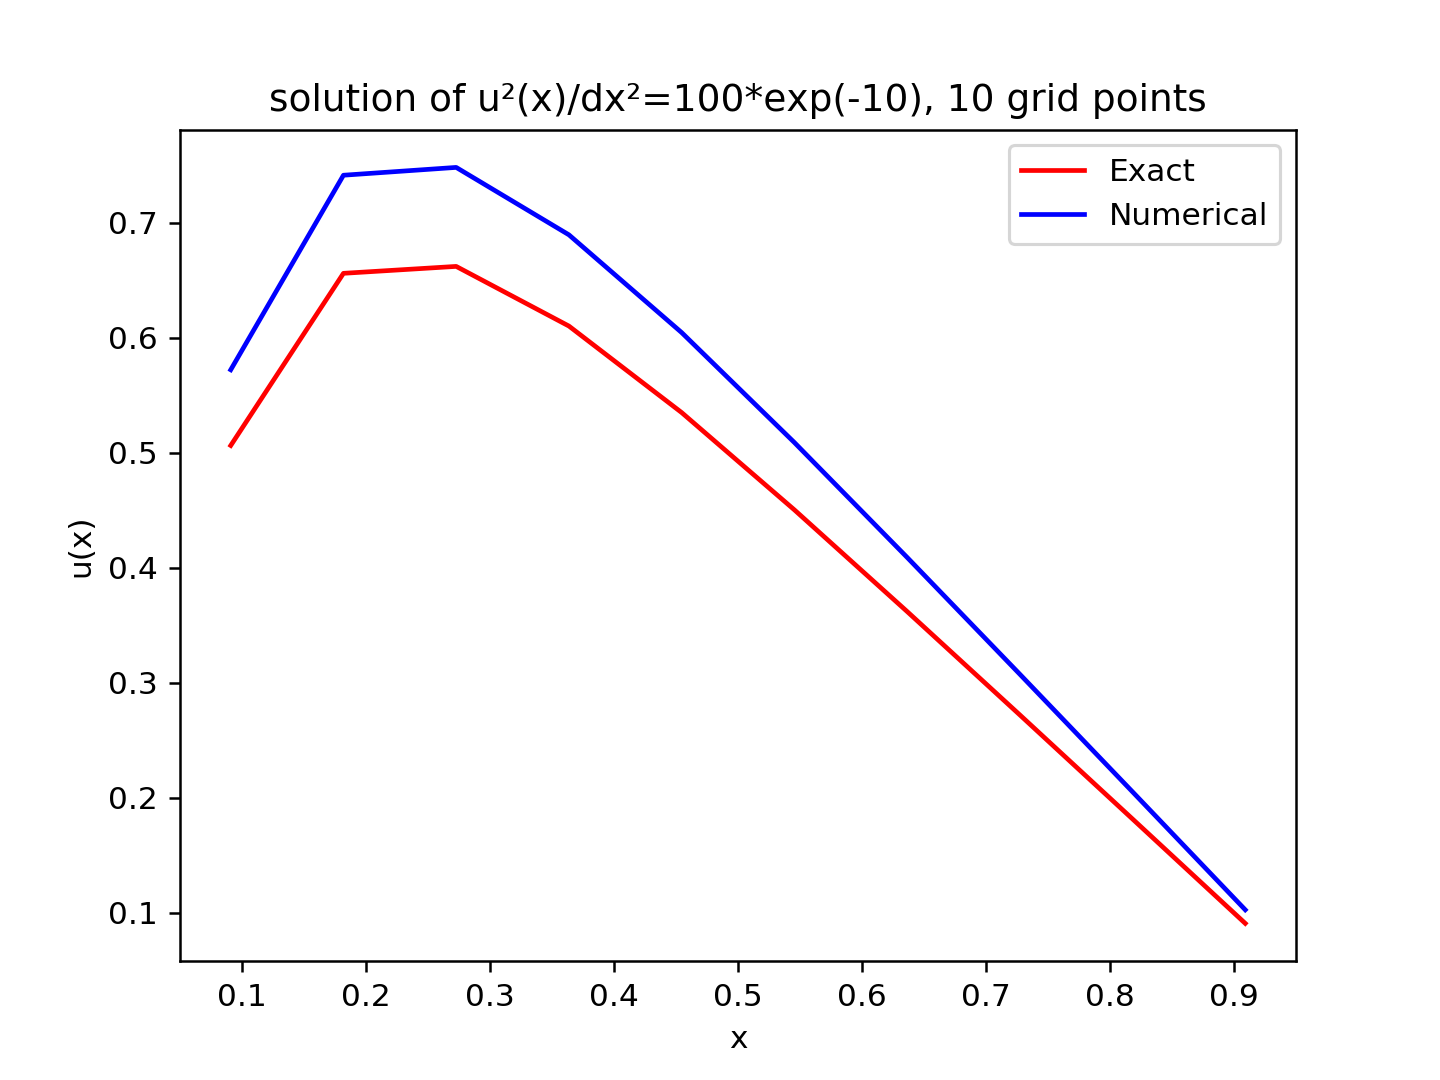
\includegraphics[width=\linewidth]{10gridpoints.png}
  \caption{solution with 10 grid points}
  \label{fig:10 grid points}
\end{figure}

\begin{figure}
  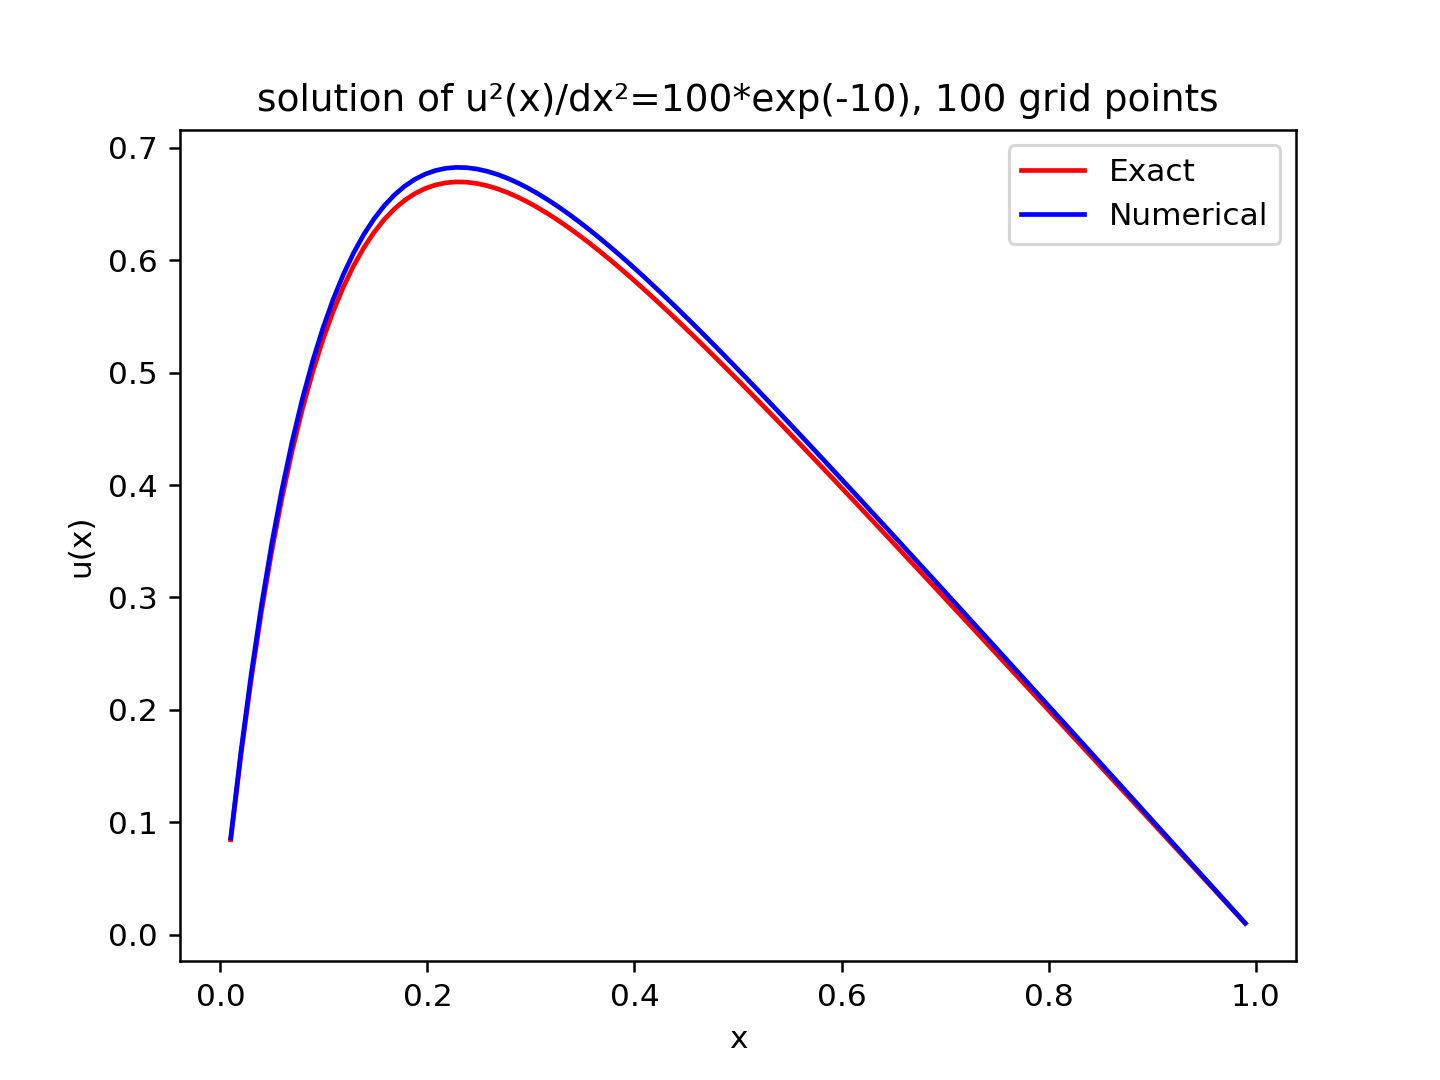
\includegraphics[width=\linewidth]{100gridpoints.png}
  \caption{solution with 100 grid points}
  \label{fig:100 grid points}
\end{figure}

\begin{figure}
  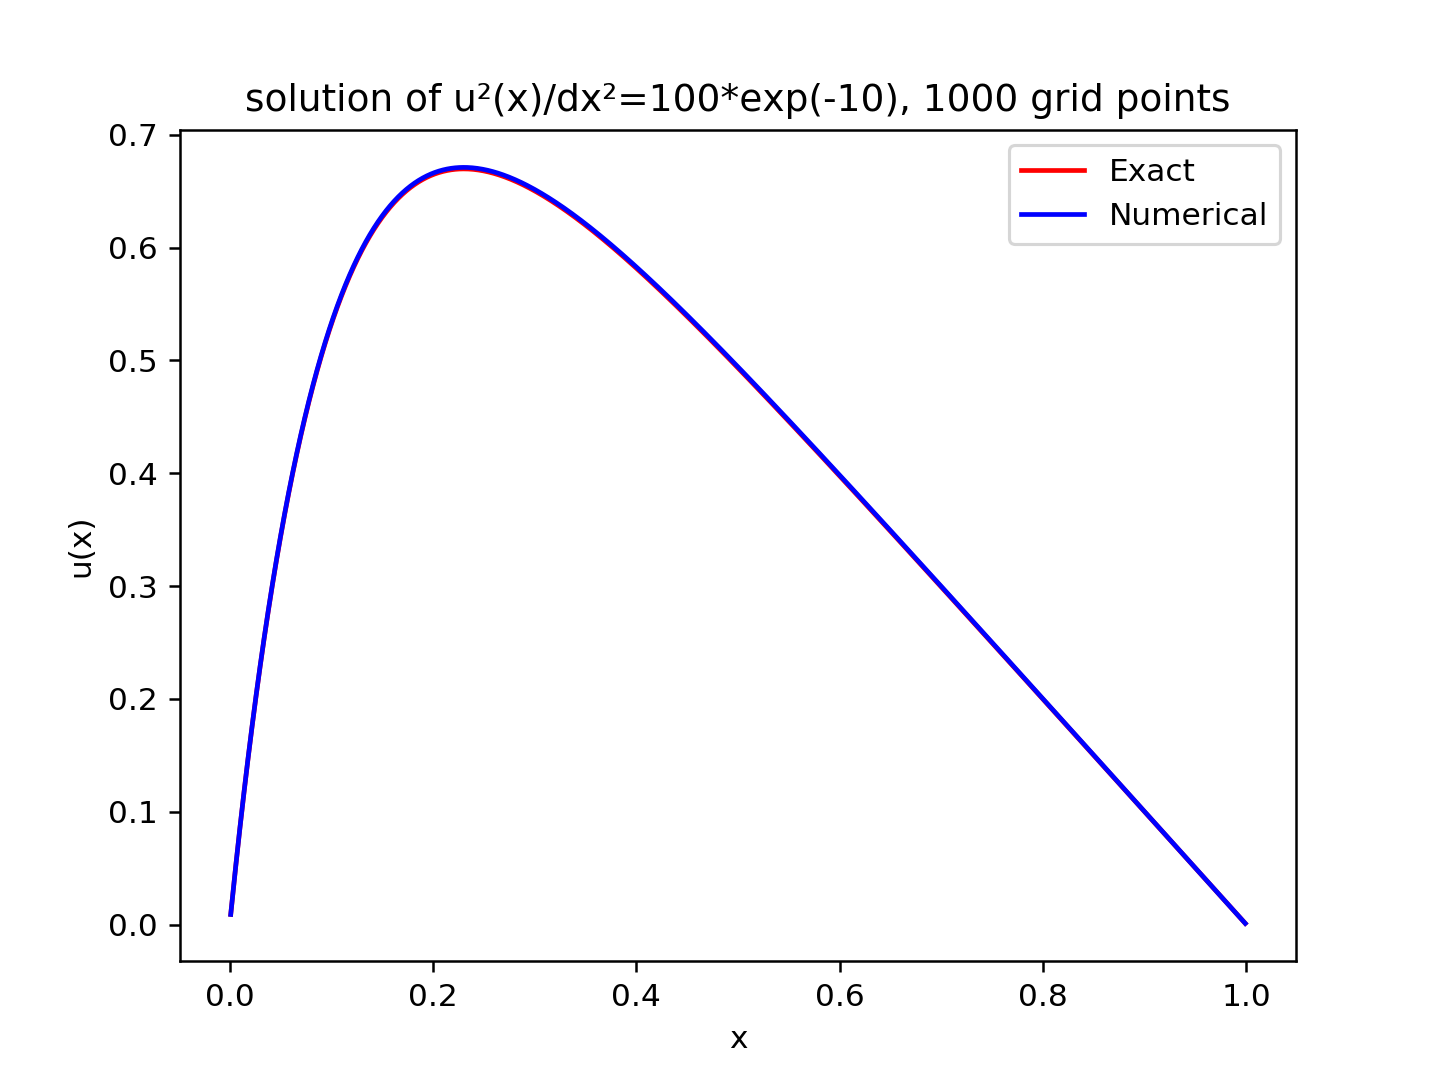
\includegraphics[width=\linewidth]{1000gridpoints.png}
  \caption{solution with 1000 grid points}
  \label{fig:1000 grid points}
\end{figure}


\subsection{Relative error and loss of numerical precision}
The specialized algorithm and the general one will give the same results, but the specialized one does not use matrices, and is therefore able to handle much higher dimensions. For this reason, I used the specialized algorithm to investigate the error. Figure 4 shows the maximum relative error as a fungtion of step length. The slope of this line is approximately 1, in contrast to the theoretical slope 2. I do not know why. Also, the relative error gets smaller for smaller step lentghs, it shows no loss of numerical precision.  This has to do with Python using double precision as default. With 64 bits, the program can handle numbers as small as $10^{-15}$. I tried to run the program with an even smaller step lenght, but that took too much time. 

In attempt of investigating the loss of numerical precision, I used used single precision for the exact solution, the input function and the numerical solution. This prodused the error plot in figure 5. The slope is still approximately 1, but around $h=10^{-5}$ somethings happens, and the relative error grows larger for smaller $h$. Here, I also got a warning about dividing by zero when $N=100 000$. This causes me to think that the increase of the error is related to underflow. 
\begin{figure}
  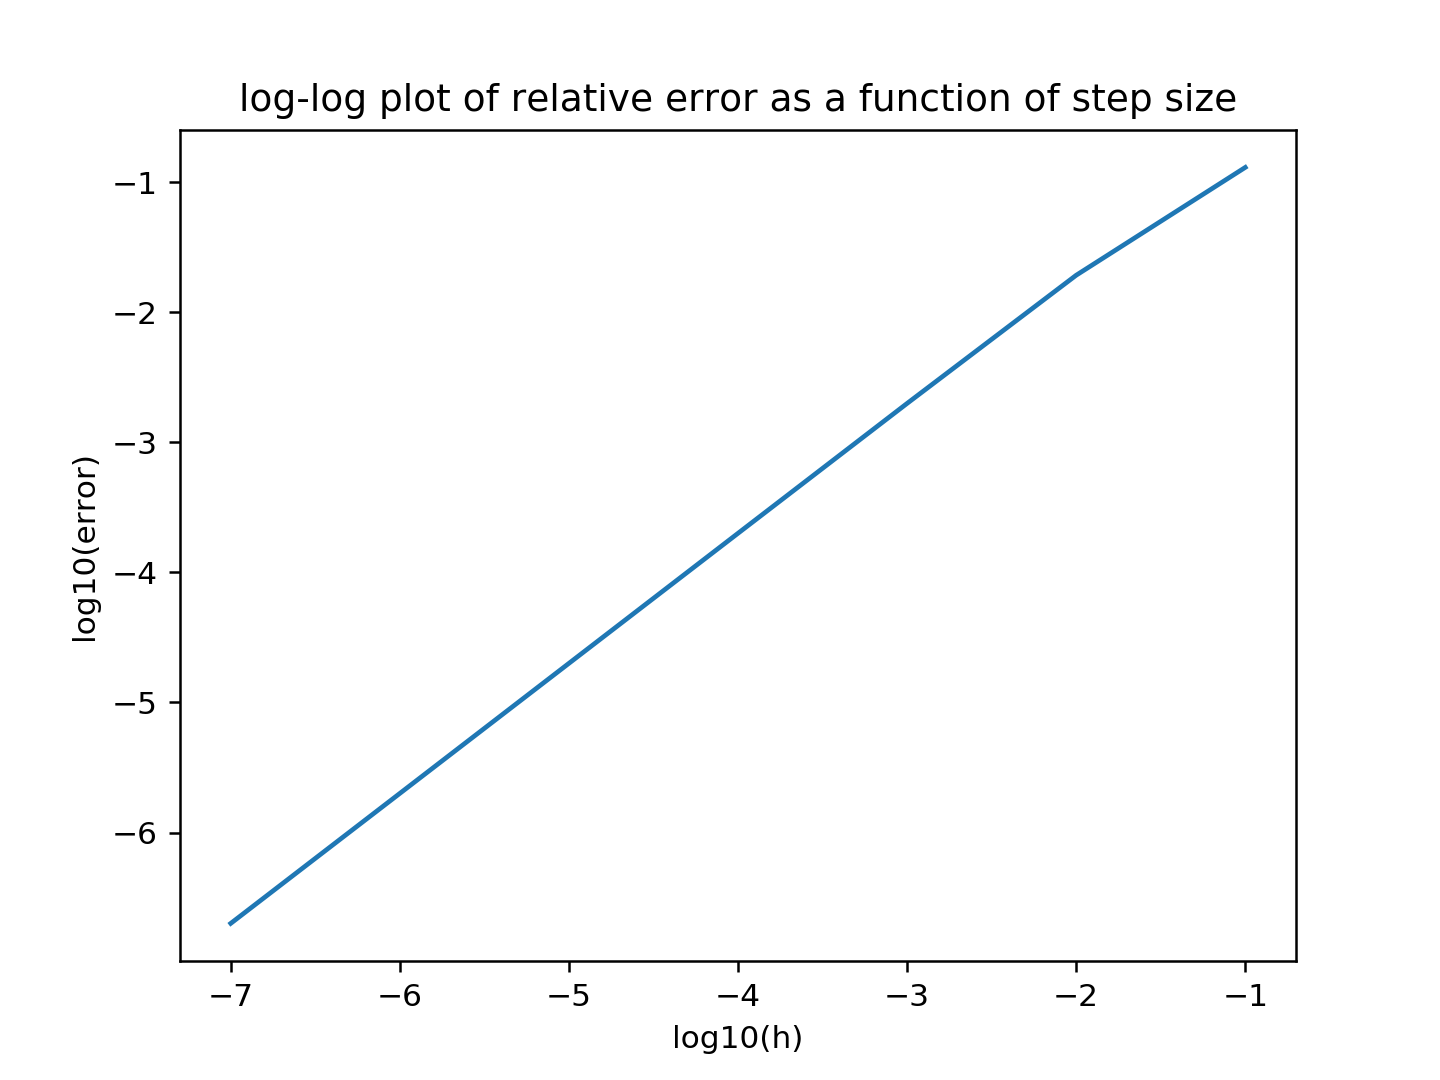
\includegraphics[width=\linewidth]{errorfigdoublefloat.png}
  \caption{Maximum relative error as a function of step length. Presicion: double}
  \label{fig:1000 grid points}
\end{figure}

\begin{figure}
  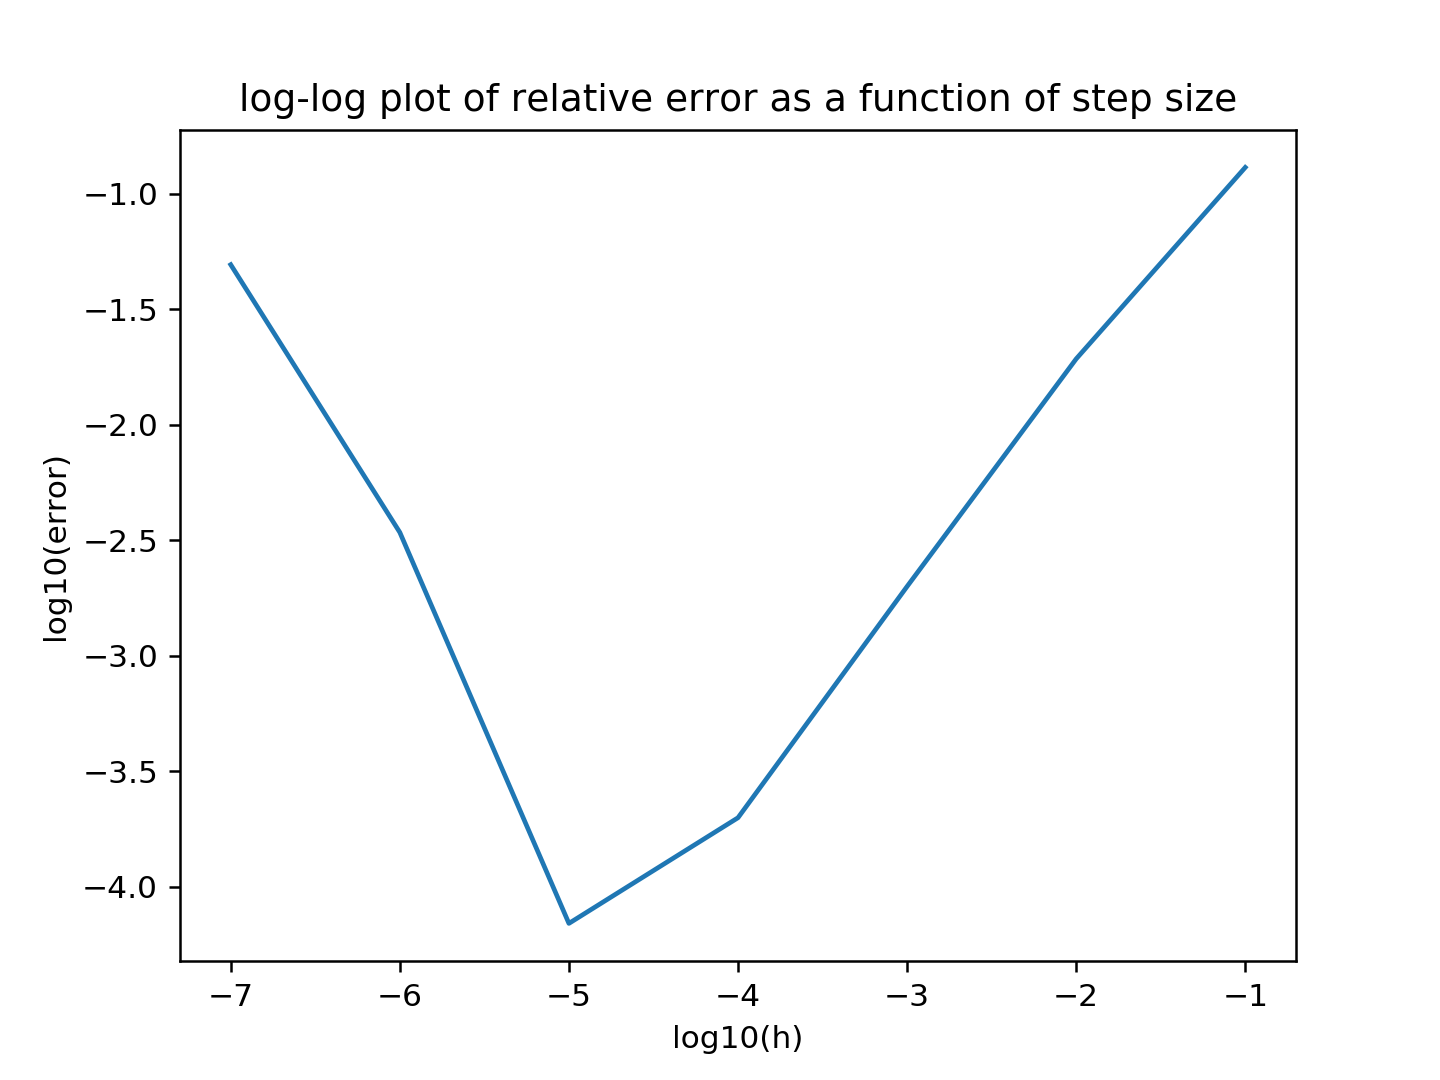
\includegraphics[width=\linewidth]{errorfigsinglefloat.png}
  \caption{Maximum relative error as a function of step length. Presicion: single}
  \label{fig:1000 grid points}
\end{figure}

\subsection{Efficiency}
In order to compare the efficiency of the algorithm for general tridiagonal matrices, the specialized algorithm and the LU decomposition in the solve function of python, I measured the CPU time. In table 1, the avreage CPU time of 5 runs is presented, along with the counted number of FLOPs for each algorithm. For all simulations, I used $N=10000$ grid points. 

When I counted the FLOPs of my 1. algorithm, I found the number to be propotional to $3N+4N^2$. This is higher than the $8N$ from the lecure notes(page 17), because my algorithm does operations on the whole row, not only on the nonzero elements. My 2. algoritm has $7N$ flops, this is because the coefficient vector is built inside the function. Else it would have 4 FLOPs. The number of flops from the LU decomposition, is taken directly from the lecture notes. I am not sure about how to compare numbers of FLOPs and CPU time in a clever way.
\begin{table}[h!]
  \centering
  \caption{CPU time and number of FLOP}
  \label{tab:table1}
  \begin{tabular}{l||c|c|c}
    method & 1. algorithm & specialized algorithm & solve function\\
    \hline
    CPU time & 500.7 ms & 13.87 ms & 22.68 s\\
    \hline
    number of FLOPs & $3N+4N^2$ & $7N$ & $\frac{2}{3}N^{3}+N^2$\\
  \end{tabular}
\end{table}



\section{Conclusion}
Finding a specialized algorithm with analytic expressions was faster and could handle higher dimensions than both a general algorithm for tridiagonal matrices and the LU decomposition. Working in Python, I had no problems with loss of numerical precision. Furter work should include a scruntiny of the slope of the relative error, as this did not follow the predicted $O(h^2)$.
\section{References}

\begin{thebibliography}{1}
\bibitem{lecturenotes} 
Hjort-Jensen, M.: Computational Physics Lectures: Linear
Algebra methods,
\\\texttt{http://compphysics.github.io/ComputationalPhysics/doc/pub/linalg/pdf/linalg-print.pdf}
\end{thebibliography}

\end{document}